\documentclass[10pt,aspectratio=169]{beamer}

\usetheme[progressbar=foot]{metropolis}
\AtBeginSection{}

\usepackage{appendixnumberbeamer}
\usepackage{booktabs}
\usepackage[scale=2]{ccicons}
\usepackage{tabularx}
\usepackage{tikz}
\usetikzlibrary{arrows.meta,positioning,shapes.geometric,fit,calc}
\usepackage{xspace}
\newcommand{\themename}{\textbf{\textsc{metropolis}}\xspace}
\usepackage{comment}
\usepackage{caption}
\usepackage[
  backend=biber,
  style=authoryear
]{biblatex}

\setbeamertemplate{bibliography item}{}
\addbibresource{bibliography.bib}

\usepackage{graphicx}
\usepackage{siunitx}



%................................................................................
% COLORS

\definecolor{ukudlaBlue}{RGB}{41, 60, 135}
\definecolor{ukudlaLightBlue}{RGB}{212, 216, 231}
\definecolor{ukudlaRed}{RGB}{164, 28, 34}
\definecolor{ukudlaLightRed}{RGB}{236, 209, 210}
\definecolor{ukudlaGreen}{RGB}{59, 139, 71}
\definecolor{ukudlaLightGreen}{RGB}{215, 231, 218}
\definecolor{ukudlaYellow}{RGB}{239, 198, 44}
\definecolor{ukudlaLightYellow}{RGB}{251, 243, 212}
\definecolor{white}{RGB}{255, 255, 255}
\definecolor{black}{RGB}{0, 0, 0}

\setbeamercolor{palette primary}{fg=white, bg=ukudlaGreen}
\setbeamercolor{progress bar}{fg=ukudlaRed, bg=ukudlaYellow}
\setbeamercolor{title separator}{fg=ukudlaRed, bg=ukudlaYellow}
\setbeamercolor{progress bar in head/foot}{fg=ukudlaRed, bg=ukudlaYellow}
\setbeamercolor{progress bar in section page}{fg=ukudlaRed, bg=ukudlaYellow}
\setbeamercolor{background canvas}{bg=white}
\setbeamercolor{block body}{bg=ukudlaLightGreen,fg=black}



%................................................................................
% PRESENTATION INFORMATION

\title{UKUDLA Data Science Certificate}
\subtitle{Data Visualization}
\author{Markus Mößler}
\institute{University of Hohenheim}



%................................................................................
% CUSTOM FOOTER

\makeatletter
\setbeamertemplate{progress bar in head/foot}{%
  \tikzset{metropolis@progressbar@foreground/.style={fill=ukudlaGreen}}%
  \tikzset{metropolis@progressbar@background/.style={fill=ukudlaLightGreen}}%

  \begin{tikzpicture}[overlay, x=\paperwidth, y=1cm]
    \fill[metropolis@progressbar@background]
      (0,0) rectangle (1,0.10);
    \fill[metropolis@progressbar@foreground]
      (0,0) rectangle
      ({\insertframenumber/\inserttotalframenumber},0.10);
    \node[anchor=south west, yshift=0.25cm, xshift=0.2cm]
      at (0,0)
      {\includegraphics[height=0.75cm]{./logos/UKUDLA_logo_03_white_bg.pdf}};
    % current section
    \ifnum\value{section}>0
      \node[
        anchor=south east,
        yshift=0.22cm,
        xshift=-0.60cm,
        fill=ukudlaLightGreen,
        rounded corners=2pt,
        inner xsep=6pt,
        inner ysep=3pt,
        font=\scriptsize\bfseries,
        text=ukudlaRed
      ] at (1,0) {
        \insertsectionhead
      };
    \fi

  \end{tikzpicture}%
}
\makeatother



%................................................................................
% CUSTOM TITLE PAGE

\makeatletter
\setbeamertemplate{title page}{
  \begin{beamercolorbox}[sep=8pt, center, wd=\paperwidth, ht=0.5\paperheight]{title page top}
    \begin{minipage}[c]{1.00\textwidth}
      \raggedleft
      \includegraphics[height=1.00cm]{./logos/ukudla_universities.pdf}
      \vspace*{0.2cm}
    \end{minipage}
    \begin{beamercolorbox}[wd=0.9\paperwidth, sep=12pt, left]{top box}
      {\usebeamerfont{title}\usebeamercolor[fg]{title}\inserttitle\par}
      \vskip0.1cm
      {\usebeamerfont{subtitle}\usebeamercolor[fg]{subtitle}\insertsubtitle\par}
    \end{beamercolorbox}
  \end{beamercolorbox}
  \begin{beamercolorbox}[sep=8pt, center, wd=\paperwidth, ht=0.5\paperheight]{title page bottom}
    \begin{beamercolorbox}[wd=0.9\paperwidth, sep=12pt, left]{bottom box}
      \hbox{%
        \hspace*{1em}
        \begin{minipage}[c]{0.40\textwidth}
          \vskip1.0cm
          {\usebeamerfont{author}\usebeamercolor[fg]{author}\insertauthor\par}
          \vskip0.1cm
          {\usebeamerfont{institute}\usebeamercolor[fg]{institute}\insertinstitute\par}
        \end{minipage}%
        \hspace*{1.5cm}
        \begin{minipage}[c]{1.00\textwidth}
          \includegraphics[height=2.0cm]{./logos/UKUDLA_logo_05.pdf}
        \end{minipage}%
      }
    \end{beamercolorbox}
    \begin{minipage}[r]{1.00\textwidth}
      \centering
      \includegraphics[width=1.00\textwidth]{./logos/ukudla_sponsors.pdf}
    \end{minipage}
  \end{beamercolorbox}
}
\makeatother

\setbeamercolor{title page top}{bg=white}
\setbeamercolor{top box}{bg=ukudlaGreen}
\setbeamercolor{title page bottom}{bg=white}
\setbeamercolor{bottom box}{bg=ukudlaLightGreen}
\setbeamercolor{title}{fg=white}
\setbeamercolor{subtitle}{fg=white}
\setbeamercolor{author}{fg=black}
\setbeamercolor{institute}{fg=black}
\setbeamercolor{date}{fg=black}



%................................................................................
% DOCUMENT

\begin{document}

\maketitle

%--------------------------------------------------
{
\setbeamertemplate{frame numbering}[none]

\begin{frame}[noframenumbering]{Table of contents}

  \small
  \setbeamertemplate{section in toc}[sections numbered]
  \tableofcontents[hideallsubsections]

\end{frame}
}
%--------------------------------------------------



\section{Motivation}


%--------------------------------------------------
% CONTENT SLIDE 1/10
\begin{frame}{Prepared data do not reveal their patterns by themselves}

\small

\begin{columns}[T]

\column{0.47\textwidth}

\textbf{A table preserves exact values}

\begin{itemize}
  \item study units and occasions are explicit;
  \item units and variables are documented;
  \item observations can be queried; and
  \item computations are reproducible.
\end{itemize}

\column{0.48\textwidth}

\textbf{A visual representation can reveal}

\begin{itemize}
  \item distributions and unusual values;
  \item differences between groups or units;
  \item change over time; and
  \item relationships between variables.
\end{itemize}

\end{columns}

\vspace{0.35cm}

\begin{beamercolorbox}[rounded=true,sep=8pt]{block body}
Data visualization maps documented observations to visual properties so that patterns can be inspected and communicated.
\end{beamercolorbox}

\end{frame}
%--------------------------------------------------


%--------------------------------------------------
% CONTENT SLIDE 2/10
\begin{frame}{A chart is an analytical argument}

\small
\centering

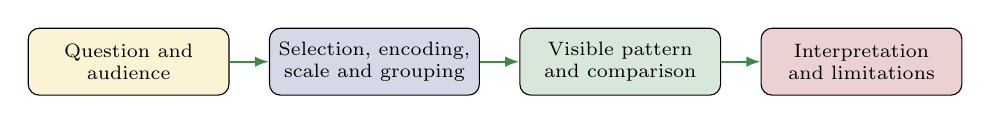
\begin{tikzpicture}[
  artifact/.style={
    draw,
    rounded corners,
    minimum width=2.55cm,
    minimum height=0.85cm,
    align=center,
    font=\scriptsize
  },
  arrow/.style={-{Latex[length=1.8mm]},thick,ukudlaGreen}
]
  \node[artifact,fill=ukudlaLightYellow] (question) {Question and\\audience};
  \node[artifact,fill=ukudlaLightBlue,right=0.50cm of question] (choices) {Selection, encoding,\\scale and grouping};
  \node[artifact,fill=ukudlaLightGreen,right=0.50cm of choices] (graphic) {Visible pattern\\and comparison};
  \node[artifact,fill=ukudlaLightRed,right=0.50cm of graphic] (claim) {Interpretation\\and limitations};
  \draw[arrow] (question) -- (choices);
  \draw[arrow] (choices) -- (graphic);
  \draw[arrow] (graphic) -- (claim);
\end{tikzpicture}

\vspace{0.50cm}

\raggedright

\begin{itemize}
  \item Exploratory graphics support investigation and iteration.
  \item Explanatory graphics focus attention on a defensible message.
  \item Both depend on choices about inclusion, aggregation and visual encoding.
  \item Neither turns an association into a causal effect.
\end{itemize}

\vspace{0.15cm}

\begin{beamercolorbox}[rounded=true,sep=8pt]{block body}
This session moves from \textbf{motivation}, through essential \textbf{concepts}, to a reproducible \textbf{application} in an analytical workflow.
\end{beamercolorbox}

\end{frame}
%--------------------------------------------------



\section{Concepts}


%--------------------------------------------------
% CONTENT SLIDE 3/10
\begin{frame}{Start with the analytical question}

\scriptsize

\begin{tabularx}{\textwidth}{lXX}
\toprule
\textbf{Question} & \textbf{Relevant structure} & \textbf{Possible graphic} \\
\midrule
How are values distributed? & One quantitative variable & Histogram, density plot, boxplot \\
How do groups compare? & Quantitative value and category & Aligned points, boxplots, faceting \\
How does a measure change? & Quantitative value ordered by time & Line or point plot \\
How do two measures vary together? & Two quantitative variables & Scatterplot \\
Where does a measure occur? & Measure and valid spatial geometry & Map \\
\bottomrule
\end{tabularx}

\vspace{0.40cm}

\small

\begin{beamercolorbox}[rounded=true,sep=8pt]{block body}
Choose a graphic from the question and variable types---not from a menu of decorative chart forms.
\end{beamercolorbox}

\end{frame}
%--------------------------------------------------


%--------------------------------------------------
% CONTENT SLIDE 4/10
\begin{frame}{Build a graphic from explicit components}

\small
\centering

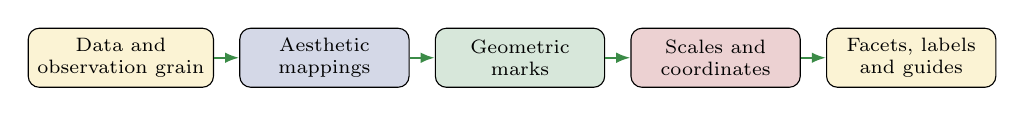
\begin{tikzpicture}[
  component/.style={
    draw,
    rounded corners,
    minimum width=2.15cm,
    minimum height=0.75cm,
    align=center,
    font=\scriptsize
  },
  arrow/.style={-{Latex[length=1.8mm]},thick,ukudlaGreen}
]
  \node[component,fill=ukudlaLightYellow] (data) {Data and\\observation grain};
  \node[component,fill=ukudlaLightBlue,right=0.32cm of data] (mapping) {Aesthetic\\mappings};
  \node[component,fill=ukudlaLightGreen,right=0.32cm of mapping] (geom) {Geometric\\marks};
  \node[component,fill=ukudlaLightRed,right=0.32cm of geom] (scale) {Scales and\\coordinates};
  \node[component,fill=ukudlaLightYellow,right=0.32cm of scale] (guide) {Facets, labels\\and guides};
  \draw[arrow] (data) -- (mapping);
  \draw[arrow] (mapping) -- (geom);
  \draw[arrow] (geom) -- (scale);
  \draw[arrow] (scale) -- (guide);
\end{tikzpicture}

\vspace{0.55cm}

\raggedright

\begin{itemize}
  \item Map variables to position, colour, shape, size or grouping.
  \item Select marks---points, lines, bars or areas---that support comparison.
  \item Use faceting when small multiples clarify group differences.
  \item Add labels and annotations that make definitions and units visible.
\end{itemize}

\vspace{0.15cm}

\centering
\textcolor{ukudlaRed}{In \texttt{ggplot2}, every visible element should follow from an explicit layer or mapping.}

\end{frame}
%--------------------------------------------------


%--------------------------------------------------
% CONTENT SLIDE 5/10
\begin{frame}{Use the strongest encodings for important comparisons}

\small

\begin{columns}[T]

\column{0.46\textwidth}

\textbf{Usually easier to compare}

\begin{enumerate}
  \item position on a common scale;
  \item position on aligned scales;
  \item length; and
  \item angle or area.
\end{enumerate}

\column{0.49\textwidth}

\textbf{Use with care}

\begin{itemize}
  \item colour hue distinguishes categories;
  \item colour lightness can show order;
  \item size is read through area, not radius;
  \item shape supports few categories; and
  \item redundant cues improve accessibility.
\end{itemize}

\end{columns}

\vspace{0.35cm}

\begin{beamercolorbox}[rounded=true,sep=8pt]{block body}
Encode the quantity that matters most with position when possible; reserve colour and size for distinctions they can carry reliably.
\end{beamercolorbox}

\end{frame}
%--------------------------------------------------


%--------------------------------------------------
% CONTENT SLIDE 6/10
\begin{frame}{Scales and aggregation change what the viewer sees}

\scriptsize

\begin{tabularx}{\textwidth}{lXX}
\toprule
\textbf{Choice} & \textbf{Risk} & \textbf{Review question} \\
\midrule
Axis limits & Differences appear exaggerated or observations disappear & Does the scale support an honest comparison? \\
Transformation & Distances acquire a different interpretation & Is a log or other scale named and justified? \\
Aggregation & Within-group variation becomes invisible & What grain and summary rule produced each mark? \\
Binning & Distribution shape changes with break placement & Are conclusions stable across reasonable bins? \\
Overplotting & Dense observations conceal frequency & Would transparency, jitter, bins or facets help? \\
Free facet scales & Shapes are comparable but magnitudes are not & Does each panel need the same quantitative scale? \\
\bottomrule
\end{tabularx}

\vspace{0.38cm}

\small

\begin{beamercolorbox}[rounded=true,sep=8pt]{block body}
Never hide a consequential filtering, transformation or aggregation decision in plotting code.
\end{beamercolorbox}

\end{frame}
%--------------------------------------------------


%--------------------------------------------------
\section{Application}
% CONTENT SLIDE 7/10

\begin{frame}{Design for interpretation, access and reuse}

\small

\begin{columns}[T]

\column{0.47\textwidth}

\textbf{Make meaning visible}

\begin{itemize}
  \item informative title and subtitle;
  \item axis labels with units;
  \item readable legends or direct labels;
  \item source and aggregation note; and
  \item annotation of the intended comparison.
\end{itemize}

\column{0.47\textwidth}

\textbf{Make the figure usable}

\begin{itemize}
  \item sufficient contrast and text size;
  \item colour-blind-safe palettes;
  \item meaning not carried by colour alone;
  \item appropriate dimensions and file type; and
  \item reproducible code and stable output path.
\end{itemize}

\end{columns}

\vspace{0.35cm}

\centering
\textcolor{ukudlaRed}{A self-contained figure states what is shown, how it was measured and what it cannot establish.}

\end{frame}
%--------------------------------------------------



%--------------------------------------------------
% CONTENT SLIDE 8/10
\begin{frame}{Ask complementary questions of prepared data}

\small

\begin{columns}[T]

\column{0.47\textwidth}

\textbf{One outcome across a study}

\begin{itemize}
  \item distribution of the outcome;
  \item differences between treatments, sites or groups;
  \item change over time or measurement order; and
  \item unusual units or measurement occasions.
\end{itemize}

\column{0.47\textwidth}

\textbf{Outcome and a second variable}

\begin{itemize}
  \item distribution and patterns of the second variable;
  \item outcome versus predictor;
  \item differences across relevant groups; and
  \item possible non-linearity or overplotting.
\end{itemize}

\end{columns}

\vspace{0.35cm}

\begin{beamercolorbox}[rounded=true,sep=8pt]{block body}
Each chart should state its observation grain: one mark may represent a sample, plot, visit, reported entity, group summary or aggregated bin.
\end{beamercolorbox}

\end{frame}
%--------------------------------------------------


%--------------------------------------------------
% CONTENT SLIDE 9/10
\begin{frame}{Turn an exploratory plot into a communication graphic}

\small
\centering

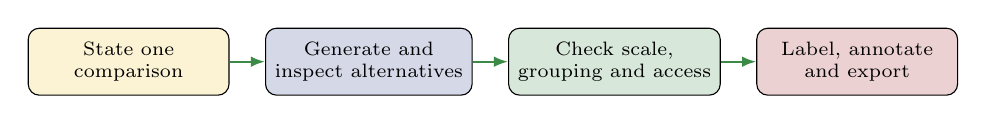
\begin{tikzpicture}[
  artifact/.style={
    draw,
    rounded corners,
    minimum width=2.55cm,
    minimum height=0.85cm,
    align=center,
    font=\scriptsize
  },
  arrow/.style={-{Latex[length=1.8mm]},thick,ukudlaGreen}
]
  \node[artifact,fill=ukudlaLightYellow] (question) {State one\\comparison};
  \node[artifact,fill=ukudlaLightBlue,right=0.45cm of question] (draft) {Generate and\\inspect alternatives};
  \node[artifact,fill=ukudlaLightGreen,right=0.45cm of draft] (review) {Check scale,\\grouping and access};
  \node[artifact,fill=ukudlaLightRed,right=0.45cm of review] (deliver) {Label, annotate\\and export};
  \draw[arrow] (question) -- (draft);
  \draw[arrow] (draft) -- (review);
  \draw[arrow] (review) -- (deliver);
\end{tikzpicture}

\vspace{0.50cm}

\raggedright

\begin{itemize}
  \item Begin with a trend, distribution or relationship plot tied to one question.
  \item Compare faceting, grouping and scale choices against the intended question.
  \item Remove decoration that does not carry information.
  \item Add units, study context, alignment rules and a non-causal interpretation.
  \item Save the figure through code rather than manual export.
\end{itemize}

\end{frame}
%--------------------------------------------------


%--------------------------------------------------
\section{Key Message}
% CONTENT SLIDE 10/10

\begin{frame}{Key message: every visual choice shapes interpretation}

\small

\begin{columns}[T]

\column{0.47\textwidth}

\textbf{Reproducible artifacts}

\begin{itemize}
  \item plotting script;
  \item exploratory figure set;
  \item one communication-ready figure;
  \item documented output paths; and
  \item source data and package environment.
\end{itemize}

\column{0.47\textwidth}

\textbf{Review evidence}

\begin{itemize}
  \item question matches the graphic;
  \item grain, units and scales are visible;
  \item grouping and aggregation are justified;
  \item design remains accessible; and
  \item interpretation respects limitations.
\end{itemize}

\end{columns}

\vspace{0.35cm}

\begin{beamercolorbox}[rounded=true,sep=8pt]{block body}
Visualization reveals and communicates patterns; the next session quantifies distributions and associations with descriptive statistics.
\end{beamercolorbox}

\vspace{0.18cm}

\centering
\textcolor{ukudlaRed}{Show the evidence clearly---and make every consequential visual choice inspectable.}

\end{frame}
%--------------------------------------------------


%--------------------------------------------------
\begin{frame}[plain,noframenumbering]{Supported by}

  South African government and the National Research Foundation

  \begin{flushleft}
    \includegraphics[trim=0cm 0cm 0cm 0cm, clip, width=0.50\textwidth]{./logos/ukudla_south_african_sponsors.pdf}
  \end{flushleft}

  German government and the German Academic Exchange Service

  \begin{flushleft}
    \includegraphics[trim=0cm 0cm 0cm 0cm, clip, width=1.00\textwidth]{./logos/ukudla_german_sponsors.pdf}
  \end{flushleft}

\end{frame}
%--------------------------------------------------

\end{document}
